\chapter{Introduction}\label{chap:introduction}
Unmanned Aerial Vehicles (UAVs) are, nowadays, accessible to all kind of users, thanks to their agility and versatility, they can be used in a wide range of applications. For many of these it is necessary an autonomous landing of the UAV on a platform using only onboard sensors. As a matter of fact, one of the major drawback of current civil Micro Air Vehicles (MAVs) is the limited flight time: automated landing systems (along with suitable recharging platforms) enable longer UAV missions with greater autonomy.\\
Furthermore these applications often require the landing target to be moving: for example, it can be a car during a reconnaissance.Therefore the MAV must be able to perform a precise landing maneuver over a specific moving platform.\\

Highly accurate localization is required in order to allow the MAV to land precisely over the platform. Most of UAVs are equipped with a GPS which only offers a precision up to 5 meters, and landing with such an uncertain state estimation can easily lead to failure. On the other hand, many applications allow the usage of other sensors, such as onboard cameras: vision based approaches, to estimate the state both of the UAV and of the moving base, are promising in this respect.\\

In this work we present a complete framework to let a quadrotor autonomously and safely land on a moving platform using only onboard sensing and computing.\\
The main parts of the framework are:
\begin{itemize}
\item self localization and state estimation of the UAV;
\item detection, tracking and state estimation of the moving landing target;
\item dynamic trajectory planning to perform a precise and smooth land on the target.
\end{itemize}

\section{Related work}\label{sec:related_work}

During the last decades several methods where developed in order to achieve automatic landing for UAVs.
Usually, in these projects calculations are done by ground stations, which allows great processing power, but lead to restrictions in autonomy on the UAV. \\

\subsection{Landing on a static platform}
At the beginning the research is focused on landing on a static platform. \\
Hardware and techniques used to achieve the successful completion of the task were various. In \cite{saripalli2002vision}, Saripalli et al. present a vision-based autonomous landing algorithm using big vehicles that can carry industrial sensors and high performance processors. This work uses hardware very far from the one we want to use, but it one of the first approaches to find a solution to this problem.

Other works, i.e.  \cite{sharp2001vision} and \cite{lange2008autonomous}, use little UAVs with cameras, estimating the pose of the quadrotor only with respect to the landing base. This consists of a single tag, therefore these frameworks are not robust to the loss of the tag and have a very noisy state estimation for the quadrotor.\\ 
Another similar work is done by Herisse in \cite{herisse2008hovering}, where the optical flow is used for hovering flight and vertical landing control.\\
The main difference with respect to our approach is that these frameworks only tackle the landing maneuver, and the final target is always in the field of view (f.o.v) of the camera. This assumption does not hold in our case.

Other papers present theoretical algorithm to perform a smooth and precise landing, but are only tested in simulation. In \cite{tang2011uav} the authors present a landing framework based on N-points algorithm and orthogonalization to estimate the state of the aircraft. In \cite{jian2012automatic} a theoretical optical guided landing control system and its corresponding guidance control law are presented.\\

Mellinger in \cite{mellinger2010control} tackles a similar problem: landing on tilted surface on which the quadrotor must pearch. He uses a motion capture system in order to have both UAV and target state estimate. His algorithm consists 
of a precomputed trajectory followed by a position-attitude control based on the linearized model of the quadrotor.\\
An interesting part of this work is the subdivision of the task in smaller parts in which trajectories and control are different in order to increase the robustness of the whole maneuver.

\subsection{Landing on a moving platform}

More interesting for the purpose of this thesis, are researches about landing on a moving platform.\\

Wenzel in \cite{wenzel2011automatic} is performing tracking and landing on a moving base with a small quadrotor. All the experiments are indoors, because of the use of IR cameras, which are not robust to outdoor conditions, due to direct sunlight. Precise and consistent results are achieved with a platform moving both in a circular path or emulating a ship turning on water, with velocities up to \SI{0.4}{\meter \per \second}.

In \cite{lee2012autonomous} Lee et al. are using visual servoing to perform the landing maneuver. A feedback control law based on the position of the target in the camera image is derived and the method is evaluated with a landing platform moving in a straight line with velocities of up to \SI{0.07}{\meter \per \second}.
To control the quadrotor to the landing site Sliding Mode Control is used. This method can deal with non linearity of the dynamics and external modeled noise (like the model of the ground effect force). 

In \cite{Kim2016} the authors propose a method to let a quadrotor land on a moving platform which can be easily found in the image of the onboard camera using color segmentation and blob detection. More specifically the platform has a color that no other object in the environment has. Also an omnidirectional camera is used  to search for the platform in the surrounding environment. Given the measurement of the position of the camera he implements an Extended Kalman Filter (EKF) to reduce the noise and predict the future position of the target. The formulation of the EKF is oversimplified, because the platform is allowed to move only in a straight line. Once the future position is estimate, a trajectory, namely position and velocity, is computed from the initial pose of the quadrotor to the final intersection point. A velocity-attitude control is implemented to follow the trajectory without replanning.

Vlantis et. al in \cite{vlantis2015quadrotor} study the problem of landing a quadrotor on an inclined moving platform. The UAV carries a forward looking camera to detect and observe the landing platform. In order to complete the task, a discrete-time non-linear Model Predictive Controller (MPC) \cite{camacho2013model} is developed. The control algorithm optimizes both the trajectories and the time horizon, while respecting input and state constraints.\\ 
The cost function of the MPC consists of different therms weighted with dynamic coefficients (function of the relative position between UAV and moving platform). More specifically, these therms are the execution time, the state of the quadrotor (position, orientation, velocity, body-rates), the smoothness and aggressiveness of the control inputs, and other factors regarding the landing task, such as the alignment between the states of UAV and moving platform (relative position, orientation, velocity) and the fact that the center of the platform should be kept within the camera's field of view during the approaching phase.\\
The major drawback of this approach is that the MPC is computationally very expensive and it is not possible to run the algorithm on-board: a ground station that carries the huge amount of calculation that MPC requires is necessary.\\

The main conclusions from the analysis of these related works is that to design a landing framework we need:
\begin{itemize}
\item a good state estimation of both the UAV and the moving platform;
\item a subdivision of the whole task in subtasks, and a manager that decides in each moment which of these stages must be completed;
\item a MPC algorithm that control the quadrotor to complete the assigned task. The algorithm should increase the robustness updating continuously the future actions that must be applied to the UAV.
\end{itemize}

\subsection{MPC for quadrotors}

Several papers have been written on MPC applied to control of the quadrotor.

In \cite{neunertfast} Neunert et.al. present a framework for real-time, unconstrained, nonlinear MPC. The algorithm combines trajectory optimization and tracking control in a unified approach. It solves the MPC problem using repeatedly a method called Sequential Linear Quadratic, generating feedforward and feedback controls actions. This method allows agile flight maneuvers with accurate tracking. All the calculations are made on an on-board Intel i7 CPU achieving a rate slightly below \SI{40}{\Hz}. No details about the performance of such a controller with lower computational power is provided.\\

In the paper \cite{bangura2014real} Bangura presents a solution to on-board trajectory tracking control for quadrotors. The
proposed approach combines a standard control paradigm for attitude and a high-level trajectory tracking with a MPC strategy. 
In order to reduce the complexity, the system is feedback linearized obtaining an equivalent linear model to which the MPC framework can be applied. Also in this case only the computation related to MPC are done onboard.

Mueller in \cite{mueller2013model} and later in \cite{mueller2015computationally} presents a method for rapid generation and feasibility verification of trajectories for quadrotors. The motion primitives are defined by the quadrotor's initial state at time $t_0$ (position, velocity, acceleration), the desired motion duration $T$, and any combination of components of the quadrotor's position, velocity and acceleration at time $t_0+T$. The trajectory are the solution of an optimization problem which minimize a cost function related to input aggressiveness, and checks if it is feasible both with respect to input and state constraints. Millions of motion primitives can be generated and evaluated per second, and so the best feasible one can be picked and followed.\\


%This final paper is very promising for our purpose because our problem can be exactly be expressed as the one solved by the algorithm proposed, and also because it is computationally inexpensive and so it is possible to run the entire code directly onboard.\\ Furthermore it is possible to use this code in an MPC-style: we have a controller with rate $\frac{1}{dt}$, at initial time $t_0$ the entire trajectory (from $t_0$ to $t_0 + T$) is calculated but only the first desired state of the trajectory (related to time $t_0+dt$) is considered, then at the next control cycle we repeat the procedure calculating the trajectory from $t_0 + dt$ to $t_0 + T$, and so on.

Table \ref{tab_1} summarizes the work done in previous research on this topic.


\newcolumntype{P}[1]{>{\centering\arraybackslash}p{#1}}
\definecolor{my_red}{rgb}{0.6350, 0.0780 ,0.1840}
\definecolor{my_green}{rgb}{0,0.5, 0}
\newcommand{\cmark}{\color{my_green} \ding{51}}
\newcommand{\xmark}{\color{my_red} \ding{55}}


\begin{center}
    \begin{tabular}{|p{4.2cm}|P{1.4cm}|P{1.4cm}|P{1.4cm}|P{1.4cm}|}
    \hline
                                                      &\color{black}\textbf{Lee} 2012  &\color{black} \textbf{Wenzel} 2011  &\color{black} \textbf{Kim} 2016 & \color{black}\textbf{Vlantis} 2015\\ \hline
    \color{black}\textbf{velocity platform} [m/s] & \color{my_red}  \textbf{0.07} & \color{my_red} \textbf{0.4} & \color{my_red} \textbf{0.5} & \color{my_red} \textbf{0.5} \\ \hline
   \color{black}\textbf{outdoor testing}             & \xmark     & \xmark         & \cmark     & \cmark \\ \hline
   \color{black}\textbf{quad indip. state estim.}     & \xmark     & \xmark         & \cmark     & \cmark \\ \hline
   \color{black} \textbf{platform state estim.}    & \xmark    & \xmark         & \xmark     & \cmark \\ \hline
    \color{black}\textbf{replanning}                   & \xmark    & \xmark          & \xmark    & \cmark \\ \hline
   \color{black}\textbf{onboard computation}  & \xmark    & \cmark          & \xmark      &\xmark \\
    \hline
    \end{tabular}
     \captionof{table}{Summary table of the results achieved in previous works on autonomous landing on a moving platform.}
     \label{tab_1}
\end{center}


%Nonlinear Tracking and landing controller for quadrotor aerial robots
%Attitude - velocity controllers
%Attitude controller: with the desired angles calculate ui* with linear eq and then nonlinear control ui from eq (8) 
%Velocity control: given desired velocity computes the desired angles and control u1 with nonlinear function (12-15)
%Model with also gyroscopic torques of the rotors then neglected
%Dynamic of the angles approximate with roll, pitch and yaw little??
%Feedback linearize 
%Landing with two different control-landing (height of base and its velocities considered as disturbances)
%z direction -> stabilize the uav at a setpoint (approach 5m, then 0m) PD controller linear
%x,y plane distance -> 0 knowing velocity x-y of the base, distance and angle between the two body frames calculate nonlinear %control  (24-25) that brings system to converge to the desired point, this control are velocity in x-y direction to give to velocity control\\

%Feedback Linearization vs. Adaptive Sliding Mode Control for a Quadrotor Helicopter 
%Need adaptive control to compensate ground effect (unknown perturbation)
%Feedback linearization
%Sliding model control to compensate the ground effect uncertantain

%Precise Quadrotor Autonomous Landing with SRUKF Vision Perception
%Not very interesting, only estimation part, controller is done with PID without any new stuffs near the ground they only estimate the velocity of the quadrotor and no the position, because the second one is difficult (easy to lose the tag)

%Coordinate landing of a quadrotor on a skid-steered ground vehicle in the presence of time delays
%Their model of the UAV dynamics are incomplete for the angular accelerations
%Control both UAV and vehicle on the ground
%Feedback linearize the system define as output x,y,x,psi
%Joint decentralized control -> exponential stabilization of the particular set of dynamics to drive relative position error to 0


\section{MBZIRC challenge}\label{chap:thechallenge}
The main reason for the development of this thesis is the participation in the Mohamed Bin Zayed International Robotics Challenge \cite{challenge_description}. MBZIRC is an international robotics competition, held every two years, that provides an ambitious and technologically demanding set of challenges, that aim at inspiring the future of robotics.\\ 
%In the description of the competition they motivate the challenge claiming that robotics have an increasing impact in a variety of new markets and on various human social aspects (for example disaster response, oil and gas, manufacturing, construction and household chores) and MBZIRC should lay the foundations of technologies for such applications include robots working more autonomously in dynamic, unstructured environments, while collaborating and interacting with other robots and humans. \\

The competition is composed of 3 challenges and in this thesis we develop a framework to complete challenge number 1 which consists in an UAV landing on a moving ground vehicle. 
The specifications of the challenge are:
\begin{itemize}
\item Max Duration:  20 minutes;
\item UAV initial condition: the participating team positions the UAV in stationary mode on the ground at the start location;
\item UGV initial condition: the ground vehicle is driven into the arena and placed at a random location along the track.
\end{itemize}


\subsection{The arena}
The challenge will be performed in an arena with the following characteristics \ref{fig:arenachallenge}:
\begin{itemize}
\item Outdoor open arena with GPS access.
\item Dimension: approximate  \SI{100}{\meter} $\times$  \SI{60}{\meter};
\item Track: width  \SI{3}{\meter}, in the shape of a figure 8 (or infinity shape), with boundary marked with white paint.
\item Terrain: relatively smooth;
\item UAV initial start location:  \SI{10}{\meter} away from the arena.
\end{itemize}

\begin{figure}[!htbp]
    \centering
    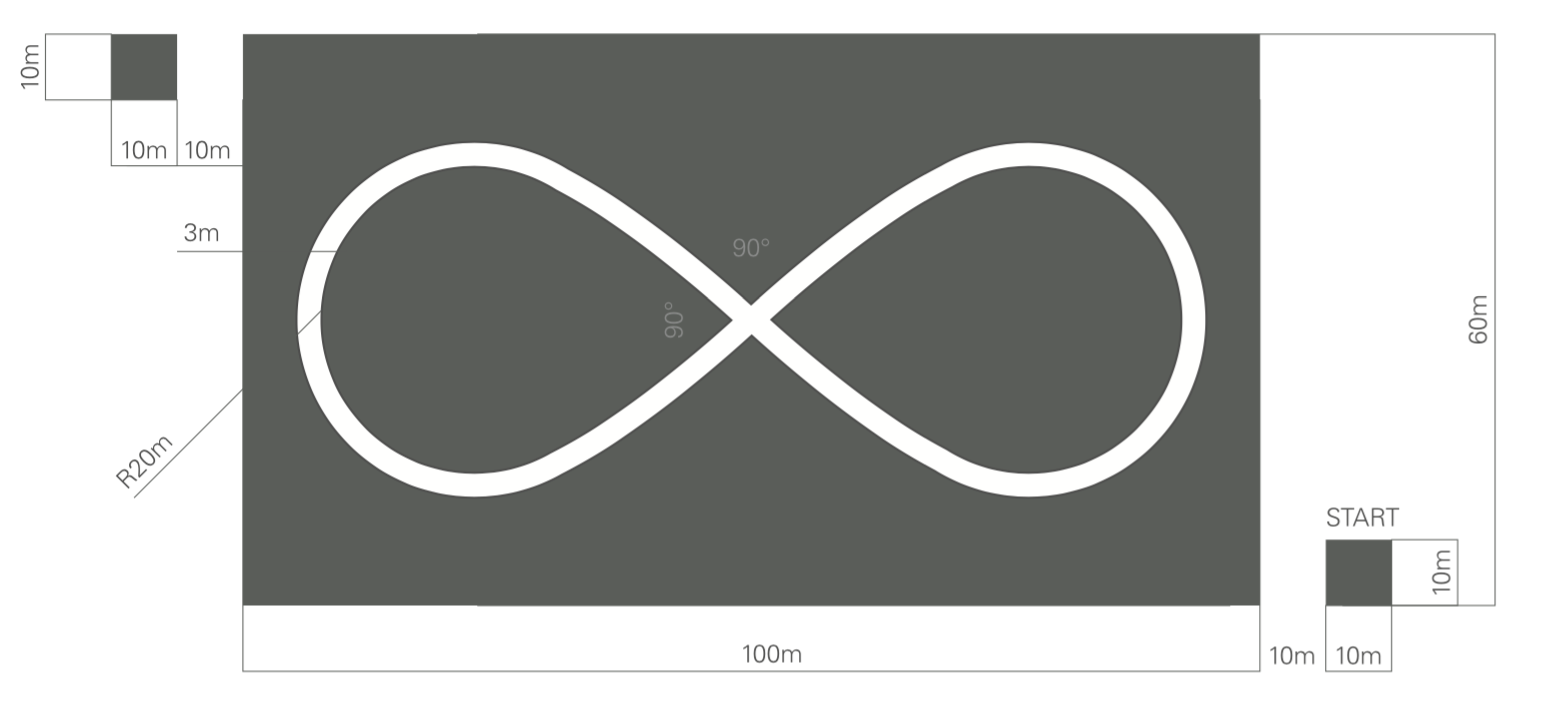
\includegraphics[width=1\textwidth]{img/arena.png}
    \caption{Arena of the challenge}
    \label{fig:arenachallenge}
\end{figure}

\subsection{Landing platform}
The landing platform is mounted on a ground vehicle of approximate dimensions  \SI{2.5}{\meter} $\times$  \SI{1.5}{\meter} $\times$  \SI{1.5}{\meter}. The moving car starts at a constant speed of \SI{15}{\km \per \hour}, then it reduces the speed to \SI{6}{\km \per \hour} after 6 minutes and to \SI{5}{\km \per \hour} after 12 minutes.\\
The landing platform is made of a ferrous surface to enable docking using magnetic or suction units.
It is a square of dimensions \SI{1.5}{\meter} $\times$  \SI{1.5}{\meter}, and approximately \SI{1.5}{\meter} above ground, positioned above the vehicle. \\
The landing zone inside the landing area is a circle of \SI{1}{\meter} diameter. The center of the circle is indicated by a cross. The landing area, the landing zone and the cross are shown in \ref{fig:finalplatform}.\\
A landing is considered successful when the point of contact of the UAV is within the landing circle, with propulsion off and rotors not spinning.\\

\begin{figure}[!htbp]
    \centering
    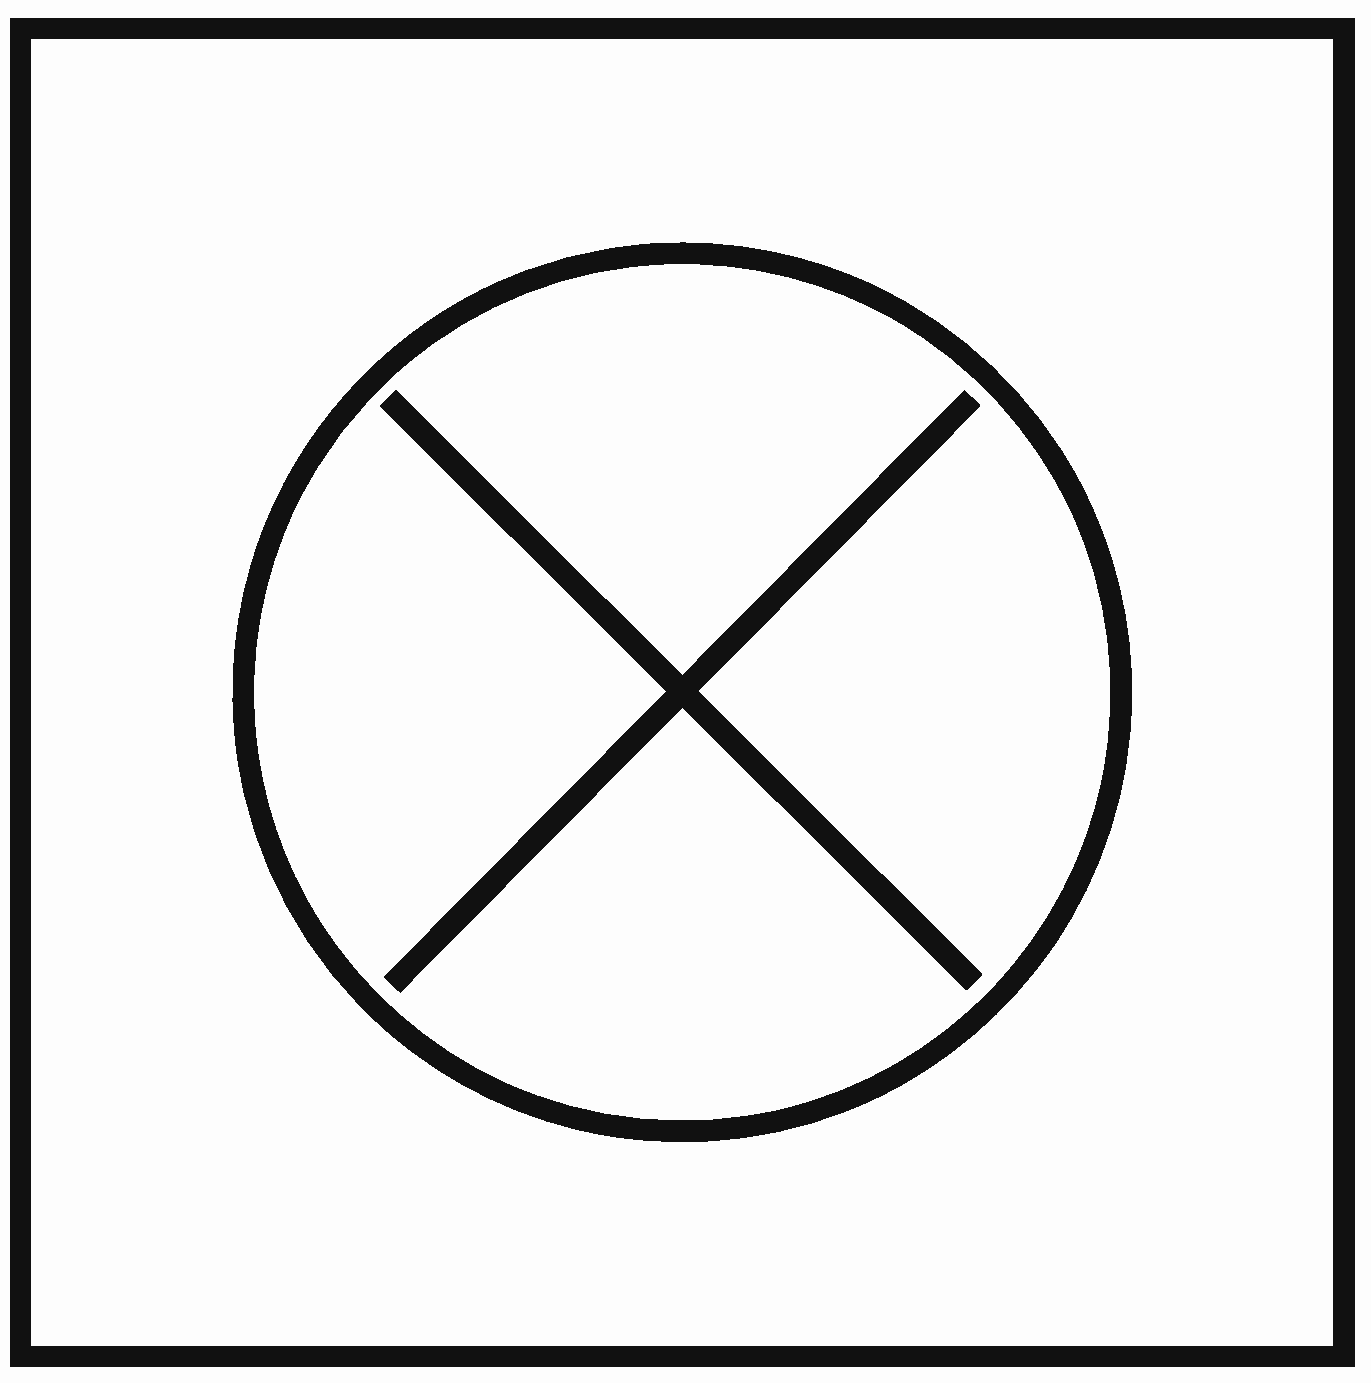
\includegraphics[width=0.4\textwidth]{img/base.pdf}
    \caption{Design of the platform in which the quadrotor must land on}
    \label{fig:finalplatform}
\end{figure}


